\documentclass[12pt]{article}
\usepackage{mathtools,amssymb}
\usepackage{graphicx,enumitem,fullpage,tikz}
\usepackage{multicol}

\title{Beginner Test 2}
\author{Stellenbosch Camp 2024}
\date{Wednesday 10 December 2024}

\begin{document} \maketitle

Note that the below problems are not arranged in order of difficulty.

\begin{enumerate}[topsep=2\bigskipamount,itemsep=1.4\bigskipamount]

% \subsection*{Tarryn}
% \item The sum of the reciprocals of four positive integers, not necessarily different from one another, is equal to $\dfrac{7}{10}$.
% Find the smallest sum of these four integers.

\item When he computes the sum of eleven consecutive positive integers, Alex very carelessly omits two consecutive numbers and gets a total of $9832$.
Calculate the correct total.

\item What is the largest six-digit number $\overline{x2014y}$ that is divisible by $33$?


% \subsection*{Yves}
% \item What is the smallest integer that can be multiplied by $2024$ to get a perfect square?

% \item What is the remainder when $\dfrac{x^{51}-201x}{x}$ is divided by $x+1$?

\item If the pattern continues in the same way, how many shaded blocks will be in Figure $30$?
\begin{center}
    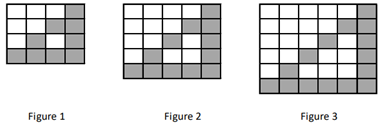
\includegraphics[scale=0.7]{fig1.png}
\end{center}

\item Find a pair $(a,b)$ of integers such that $123a +36b =3$.

\item Calculate the following product into its simplest form:
\[ \left(1 - \frac{1}{2^2}\right)\left(1 - \frac{1}{3^2}\right)\cdots \left(1 - \frac{1}{9^2}\right)\left(1 - \frac{1}{10^2}\right). \]

%\item Let $a$ and $b$ be two co-prime integers (that is; $\text{HCF}(a,b)=1)$). Show that if $ab$ is a perfect square, then both $a$ and $b$ are perfect squares.\\
%(HINT: Assume for simplicity that $a=p_1^{n_1}p_2^{n_2}$ and $b=p_3^{n_3}p_4^{n_4}$ are the prime factorizations of $a$ and $b$ respectively)


% \subsection*{Muphulusi}
\item If $a$ and $b$ are positive real numbers such that $\dfrac{a^2}{b^2}+\dfrac{b^2}{a^2} = 7$, find the value of $\dfrac{a}{b}+\dfrac{b}{a}$.

% \item Solve for $x$ if $x^{x^4} = 64$.

\item What is the value of $2023^2-2022^2$?

% \item If $a+b = 1$ and $a^2+b^2 = 2$, what is the value of $a^5+b^5$?

\item Given that $3^m-2^m = 65$, calculate the value of $m$.

\hfill (turn the page)

\pagebreak

% \subsection*{Kate}
\item
\begin{multicols}{2}
Let $ABC$ be a triangle with a right angle at $B$, such that $AB = 15$ and $BC = 20$.
Let $D$ be the point on line $AC$ such that $BD$ is perpendicular to $AC$.
Calculate the length of $BD$.
\begin{center}
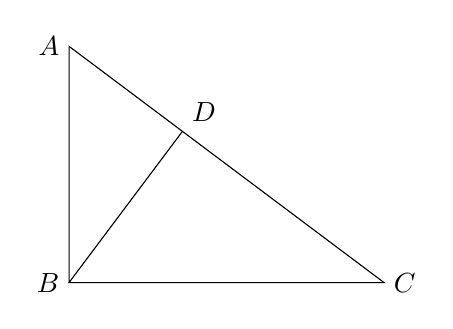
\begin{tikzpicture}[scale=0.2]
    % \path (7.2,9.6) node 
    \draw (7.2,9.6) node[above right] {$D$} -- (0,0) node[left] {$B$} -- (20,0) node[right] {$C$} -- (0,15) node[left] {$A$} -- (0,0);
\end{tikzpicture}
\end{center}
\end{multicols}

\item
\begin{multicols}{2}
In the figure, square $ABCD$ has side length $12$, square $EFGH$ has side length $6$, and both squares have the same centre.
An interesting fact is that the area of the shaded region $ABFE$ is constant and does not depend on the rotation of square $EFGH$.

What is the area of the shaded region?
\vspace*{24pt}
\columnbreak
\begin{center}
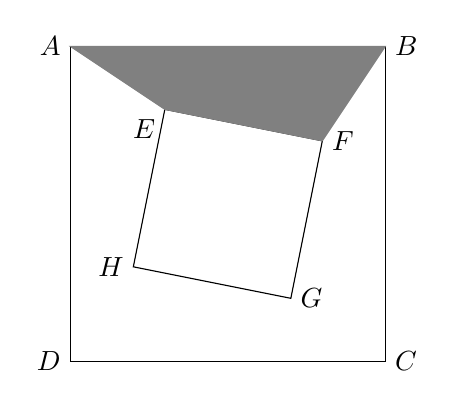
\begin{tikzpicture}[scale=0.4]
    \draw (-5,5) node[left] {$A$} -- (5,5) node[right] {$B$} -- (5,-5) node[right] {$C$} -- (-5,-5) node[left] {$D$} -- cycle;
    \draw (-2,3) node[below left] {$E$} -- (3,2) node[right] {$F$} -- (2,-3) node[right] {$G$} -- (-3,-2) node[left] {$H$} -- cycle;
    \filldraw[gray] (-5,5) -- (-2,3) -- (3,2) -- (5,5) -- cycle;
\end{tikzpicture}
\end{center}
\end{multicols}

% \item \begin{multicols}{2}
% The figure shows a square and a circle having the same centre. The sides of the square are tangents to the circle. If the perimeter of the square is 25cm, calculate the area of the circle.
% \begin{center}
%     \begin{tikzpicture}[scale=2]
%         \draw (-1,-1) -- (1,-1) -- (1,1) -- (-1,1) -- cycle;
%         \draw (0,0) circle [radius=1];
%     \end{tikzpicture}
% \end{center}
% \end{multicols}

% \item \begin{multicols}{2}
% A certain type of ring has outer diameter of 58mm, an inner diameter of 40mm and thickness of 1mm.
% If one stacks enough rings on top of each other, it is possible to stand another ring vertically on top of the pile in such a way that the ring just touches the bottom.
% How many rings are in the stack when this happens?
% \begin{center}
%     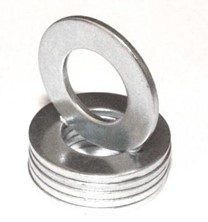
\includegraphics[width=0.3\textwidth]{Beginner/rings.jpg}
% \end{center}
% \end{multicols}


% \subsection*{Naeem}
\item If $x$ and $y$ are positive real numbers such that
\[ \sqrt{2x} +\sqrt{y} = 13 \quad\text{and}\quad \sqrt{8x} +\sqrt{9y} = 35, \]
calculate $20x+23y$.

\item Find the number of digits in the number $2 \cdot 4^{12} \cdot 5^{25}$.

\item How many pairs of integers $x$ and $y$ are there such that
\[ 0 < x < y \quad\text{and}\quad \sqrt{2024} = \sqrt{x} +\sqrt{y}? \]

% \item Which terms must be removed from the sum
% \[ \frac{1}{2} +\frac{1}{4} +\frac{1}{6} +\frac{1}{8} +\frac{1}{10} +\frac{1}{12} \]
% so that the sum of the remaining terms is $1$?


% \subsection*{Liam}
% \item Tarryn is at a restaurant and wants to have a burger, a drink, and a dessert.
% The restaurant has 10 different burgers, 4 different drinks, and 3 different desserts available.
% How many different meals could Tarryn have?

\item Tarryn is at a restaurant and wants to have at most one burger, at most one drink, and at most one dessert.
The restaurant has 10 different burgers, 4 different drinks, and 3 different desserts available.
How many different meals could Tarryn have?

\item How many different permutations are there of the letters in NAEEM?

\item Yves has a bag with $10$ stones, each of a different colour (white, black, red, green, blue, cyan, magenta, teal, grey, and purple).
He wants to take five of these stones, as long as he does not take both the white and the black stones together.
In how many ways can he do this?

\end{enumerate}

\end{document}